\documentclass{../industrial-development}
\graphicspath{{12-process-of-turning-a-developer-into-a-manager/}}

\title{Процесс превращения разработчика в~менеджера}
\author{Румянцева Мария Сергеевна, \\Феофанова Алла Александровна, \\ПИ-21 МО}
\date{}

\begin{document}

\begin{frame}
  \titlepage
\end{frame}

\section{Разработчик и менеджер}

\begin{frame} \frametitle{Разработчик и IT-менеджер}
	\alert{Разработчик} — программист, который занимается созданием различных продуктов в ИТ: компьютерных игр, мобильных приложений, веб-сайтов и др. 	\\
~\\
	\alert{IT-менеджер} – это специалист, чьей главной задачей является управление проектом в целом: проектирование и расстановка приоритетов, планирование выполнения задач, контроль, коммуникации, а также оперативное решение проблем.
\end{frame}
\lecturenotes
IT-менеджер – это специалист, чьей главной задачей является управление проектом в целом: проектирование и расстановка приоритетов, планирование выполнения задач, контроль, коммуникации, а также оперативное решение проблем.
IT-менеджеры — это сотрудники, отвечающие за качество услуг, предоставляемых пользователям (сотрудникам компании, а иногда — её клиентам и партнёрам) на базе информационных технологий.
IT-менеджер компании – сотрудник, управляющий информационными процессами. Он разбирается не только в технических аспектах IT-среды, но и в вопросах ее взаимодействия с другими сферами: финансовой, кадровой, рыночной.  Задача менеджера внутри фирмы: знать цели развития бизнеса компании, уметь представить бизнес-процессы для их автоматизации, осуществить правильный выбор информационной системы и рассчитать эффект от ее применения.  Его внешние цели – обеспечить клиентам получение качественных ИТ-услуг или организовать продажу информационных продуктов.
Специфика деятельности разработчика (другое название этой профессии — Developer) всецело зависит от выбранного направления. К примеру, разработкой программного обеспечения прикладного характера (игры‚ бухгалтерские программы‚ редакторы‚ мессенджеры, ПО для систем видео- и аудионаблюдения) занимаются прикладные программисты; созданием операционных систем, работой с сетями, написанием интерфейсов к базам данных озадачены системные программисты; воплощением в жизнь проектов веб-дизайнеров, т. е. созданием сайтов, заняты веб-программисты.
~\cite{How_to_be_a_good_IT-manager}


\begin{frame} \frametitle{Важные качества разработчика в IT}
	 \begin{itemize}
	 	\item Сильные технические навыки
		\item Аналитический склад ума
	 	\item Готовность к обучению
	 	\item Умение работать в команде
		\item Стрессоустойчивость
		\item Вовлеченность в рабочий процесс
		\item Способность к концентрации
	 \end{itemize}
\end{frame}
\lecturenotes
Сфера информационных технологий и телекоммуникаций отличается стремительным развитием, и для сохранения набранного темпа становятся всё необходимей специалисты, которые помогли бы ей в этом. В то же время, специалистам следует соответствовать определённым требованиям, без них они не смогут успешно справляться со своими профессиональными задачами. Так какие же личные качества помогают работникам в сфере IT и телекоммуникаций стать настоящими профессионалами?
Такие специалисты в первую очередь должны быть склонны к математике, информатике и работе с техникой, в том числе с компьютерами. Им необходимо иметь аналитический склад ума, хорошую память и способность работать с большим количеством информации. Также незаменимыми качествами для всех сотрудников в этой области, независимо от должности, являются ответственность, организованность, стрессоустойчивость, умение самостоятельно обучаться по специализированной литературе.
Стоит отметить, что облик IT-специалиста, работавшего, к примеру, десять лет назад, существенно отличается от современного. Теперь это не молчаливый, сосредоточенный человек, не отрывающийся от компьютера весь рабочий день, а коммуникабельный сотрудник, готовый к работе в команде и прямому диалогу с клиентами. Создавая продукт, работники IT-сферы и телекоммуникации ориентируются на его будущих потребителей, поэтому хорошо знают интересы и потребности своих потенциальных клиентов.
Важно не просто иметь все эти качества, но и грамотно себя преподносить, например, во время трудоустройства. Главная визитная карточка здесь – резюме, в нём стоит обязательно указать свои преимущества и способности. 
У обладателей таких качеств действительно много шансов найти работу по своей специальности, тем более что спрос на работников в сфере информационных технологий и телекоммуникаций заметно превышает предложение. Конечно, для того чтобы быть компетентными и востребованными им понадобится не только психологическая склонность к профессии. Им не обойтись без хорошего образования, профессиональных знаний и умений, постоянного совершенствования своих навыков. А знание английского языка, к тому же, поможет найти работу в уже известной или очень перспективной зарубежной компании.
~\cite{How_to_be_a_good_IT-manager}



\subsection{Основания для перевода разработчика в менеджера}
\begin{frame} \frametitle{Основания компании для перевода разработчика в менеджеры}
\begin{itemize}
		\item Стремление <<вырастить>> менеджера внутри компании		
		\item Отсутствие менеджера, при невозможности увеличения штата сотрудников
		\item Дефицит времени на введение в работу человека со стороны	
		\item Понимание специфики организации и отрасли
		\item Знание сильных и слабых сторон коллектива
	\end{itemize}
\end{frame}
\lecturenotes
???
~\cite{How_to_be_a_good_IT-manager}

\begin{frame} \frametitle{Необходимые качества IT-менеджера}
\begin{itemize}
		\item Лидерские качества
		\item Умение находить общий язык
		\item Знание процессов разработки и особенностей продукта изнутри
		\item Готовность взять ответственность не только за себя, но и за других
		\item Желание развиваться
		\item Доверие (авторитет) у заказчика
		\item Достижение определенных профессиональных высот

	\end{itemize}
\end{frame}
\lecturenotes
???
~\cite{How_to_be_a_good_IT-manager}

\subsection{Подготовка менеджера проекта}
\begin{frame} \frametitle{Подготовка менеджера проекта}

	 	\begin{table}[H]
\caption{\label{tab:canonsummary} Обучение специалистов}
\begin{center}
\begin{tabular}{|p{0.2\linewidth}|p{0.8\linewidth}|}
\hline
\textbf{Вид} & \textbf{Специфика} \\
\hline
Официаль-ные &  обучение специалистов в ВУЗ-ах и на специальных курсах, завершение которых удостоверяется соответствующим документом. \\
\hline
Полуофи-циальные  & прохождение краткосрочных курсов, посещение популярных лекций и практических занятий. \\
\hline
Неофициаль-ные &  участие в конференциях, семинарах и ознакомление с соответствующей литературой \\
\hline
Обучение в процессе работы & обучение на рабочем месте, а также самообразование. \\
\hline
\end{tabular}
\end{center}
\end{table} 
\end{frame}
\lecturenotes
официальные – обучение специалистов в ВУЗ-ах и на специальных курсах, завершение которых удостоверяется соответствующим документом. К слушателям этой формы подготовки предъявляются обязательные требования, как при начале, так и при завершении обучения, а в ряде случаев, и по ходу самого обучения;
полуофициальные – прохождение насыщенной программы обучения на краткосрочных курсах (продолжительностью от нескольких дней до нескольких месяцев), посещение популярных лекций и практических занятий. К слушателям этой формы подготовки не предъявляются какие-либо обязательные требования, и они не получают специальных удостоверений об их окончании;
неофициальные – участие в конференциях, симпозиумах, региональных семинарах, собраниях профессиональных обществ, а также ознакомление с соответствующей литературой;
обучение в процессе работы – это обучение на рабочем месте при выполнении конкретного проекта, а также самообразование.
~\cite{How_to_be_a_good_IT-manager}


\subsection{Отличия характера работы и стиля мышления}
\begin{frame} \frametitle{Отличия в характере работы по~традиционной методологии}

	 	\begin{table}[R]

\begin{center}
\begin{tabular}{|p{0.5\linewidth}|p{0.5\linewidth}|}
\hline
\textbf{Разработчик} & \textbf{IT-Менеджер} \\
\hline
\begin{itemize}
\item Отсутсвтует общение с заказчиком
\item Должен уметь читать чужой код и разбираться в нем
\item Направленность на решение конкретной задачи
\item Ответственен только за себя
\end{itemize}
 & 
\begin{itemize}
\item Общение с заказчиком
\item Постоянное взаимодействие с командой
\item Правильное распределение бюджета и времени сотрудников
\item Повышенная ответственность (за проект)
\end{itemize} \\
\hline
\end{tabular}
\end{center}
\end{table} 
\end{frame}
\lecturenotes
~\cite{How_to_be_a_good_IT-manager}

\begin{frame} \frametitle{Отличия в характере работы по~гибкой методологии}

	 	\begin{table}[R]

\begin{center}
\begin{tabular}{|p{0.5\linewidth}|p{0.5\linewidth}|}
\hline
\textbf{Разработчик} & \textbf{IT-Менеджер} \\
\hline
\begin{itemize}
\item 
\item 
\item 
\item 
\end{itemize}
 & 
\begin{itemize}
\item 
\item 
\item
\item
\end{itemize} \\
\hline
\end{tabular}
\end{center}
\end{table} 
\end{frame}
\lecturenotes
~\cite{How_to_be_a_good_IT-manager}


\begin{frame} \frametitle{Отличия характера работы разработчика и менеджера}
	\begin{block}{Разработчик}
\begin{itemize}
\item Отсутсвтует общение с заказчиком
\item Должен уметь читать чужой код и разбираться в нем
\item Направленность на решение конкретной задачи
\item Ответственен только за себя
\end{itemize}
\end{block}
\end{frame}
\lecturenotes

\begin{frame} \frametitle{Отличия характера работы разработчика и менеджера}
	\begin{block}{IT-менеджер}
\begin{itemize}
\item Общение с заказчиком
\item Постоянное взаимодействие с командой
\item Правильное распределение бюджета и времени сотрудников
\item Повышенная ответственность (за проект)
\end{itemize}
\end{block}
\end{frame}
\lecturenotes

~\cite{How_to_be_a_good_IT-manager}

\begin{frame} \frametitle{Отличия стиля мышления разработчика и менеджера}
	\begin{block}{Разработчик}
\begin{itemize}
\item Узкое мышление
\item Согласование изменений с teamleader и IT-менеджером
\item Глубокое погружение в свой процесс работы
\end{itemize}
\end{block}
\end{frame}
\lecturenotes

~\cite{How_to_be_a_good_IT-manager}

\begin{frame} \frametitle{Отличия стиля мышления разработчика и менеджера}
	\begin{block}{IT-менеджер}
\begin{itemize}
\item Видимость проекта в целом
\item Согласование изменений с заказчиком 
\item Мотивирует команду на результат
\end{itemize}
\end{block}
\end{frame}
\lecturenotes

\subsection{Роли менеджеров по модели РАЕI}

\begin{frame} \frametitle{Роли менеджеров — РАЕI\footnote[2]{по мнению д.~Адизеса}}
	Идеального руководителя, по мнению доктора Адизеса, не существует. Согласно его модели PAEI, для достижения эффективности руководителю нужны четыре качества: 
 \begin{itemize}
	 \item \alert{P} — производитель результатов (producer), 
	 \item \alert{A} — администратор (administrator), 
	 \item \alert{Е} — предприниматель (entrepreneur), 
	 \item \alert{I} — интегратора (integrator). 
 \end{itemize}
Все это не может сочетаться в одном человеке — в реальности менеджеры выполняют хорошо 1-2 функции. При этом одна из функций у правильного менеджера должна доминировать, а всеми остальными он должен владеть на элементарном уровне.  \\

\end{frame}
\lecturenotes
~\cite{How_to_be_a_good_IT-manage


\begin{frame} \frametitle{Производитель}
	 \begin{block}{Ключевой вопрос P:}
		ЧТО делаем?
	\end{block}	
Производитель (Р) ориентирован, в первую очередь, на результат, создание продуктов и услуг для удовлетворения потребностей покупателей. Для Р выполненная задача собственными руками, не делегируя никому, приносит наибольшее удовольствие.\\~\\ Р ориентированы на текущие потребности и зачастую не способны подняться над ситуацией вверх и посмотреть с высоты, оценить ее в полном комплексном масштабе. 
\end{frame}
\lecturenotes
~\cite{How_to_be_a_good_IT-manager}

\begin{frame} \frametitle{Администратор}
	\begin{block}{Ключевой вопрос A:}
		КАК делаем?
	\end{block}	
Администратор (А) — нацелен на оптимизацию и минимизацию использования имеющихся ресурсов. Он систематизирует весь процесс управления организацией, упорядочивает его, устанавливает бюрократический порядок, прописывает функциональные обязанности, вводит стандартизированные процедуры.\\~\\ Обожает созданные им же правила и инструкции, не терпит, когда другие нарушают их, всегда доводит начатое до конца, наряду с этим всеми силам избегает риска.
\end{frame}
\lecturenotes
~\cite{How_to_be_a_good_IT-manager}

\begin{frame} \frametitle{Предприниматель}
	\begin{block}{Ключевой вопрос E:}
		ЗАЧЕМ и КОГДА делаем?
	\end{block}	
Предприниматель (Е) предпочитает генерировать новое, экспериментировать, внедрять. Такой руководитель не дает организации останавливаться на достигнутом. Благодаря тому, что у него всегда много планов и идей, он стимулирует всех вокруг идти дальше, развиваться.\\~\\ Большое количество идей Е приводит также и к тому, что большинство из них не воплощаются, а дела, к которым такой руководитель «остыл», не доводятся до конца. 
\end{frame}
\lecturenotes
~\cite{How_to_be_a_good_IT-manager}

\begin{frame} \frametitle{Интегратор}
	\begin{block}{Ключевой вопрос I:}
		КТО делает?
	\end{block}	
Интегратор (I) — это лидер, способный создать общие традиции, ценности, корпоративную культуру организации. Он определяет общую для всех стратегическую цель, призывает трудиться всем вместе, тем самым поддерживая в организации единство. \\~\\ С ним очень приятно общаться, он объединяет людей вокруг себя. Иногда такой руководитель может быть излишне мягким.
\end{frame}
\lecturenotes
~\cite{How_to_be_a_good_IT-manager}

\begin{frame} \frametitle{Модель PAEI}
{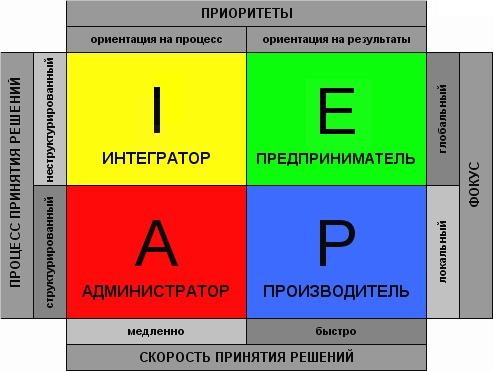
\includegraphics[width=0.95\linewidth]{paei.png}}
\end{frame}
\lecturenotes

\begin{frame} \frametitle{Примеры профилей менеджеров }
	\begin{enumerate}
\item Идеальный (несуществующий в реальности) менеджер: 
		 \begin{itemize}
                     \item Производитель — 100\%
 		 \item Администратор — 100\%
 		 \item Предприниматель — 100\%
		\item Интегратор — 100\%
		\end{itemize} 
\item Хороший менеджер-организатор:	
		 \begin{itemize}
                         \item Производитель — 20\%
 		 \item Администратор — 90\%
 		 \item Предприниматель — 30\%
		\item Интегратор — 30\%
		\end{itemize} 
\end{enumerate}
\end{frame}
\lecturenotes
~\cite{How_to_be_a_good_IT-manager}

\begin{frame} \frametitle{Примеры профилей менеджеров }
	\begin{enumerate}
\setcounter{enumi}{2}
\item Хороший менеджер-мотиватор:
		 \begin{itemize}
                     \item Производитель — 20\%
 		 \item Администратор — 10\%
 		 \item Предприниматель — 20\%
		\item Интегратор — 90\%
		\end{itemize} 
\item Менеджер-<<Трудоголик>>:	
		 \begin{itemize}
                         \item Производитель — 100\%
 		 \item Администратор — 0\%
 		 \item Предприниматель — 0\%
		\item Интегратор — 0\%
		\end{itemize} 
\end{enumerate}
\end{frame}
\lecturenotes
~\cite{How_to_be_a_good_IT-manager}

\subsection{Типы программистов}
\begin{frame} \frametitle{Типы программистов\footnote[1]{по мнению Дж.~Ханка~Рейнвотера}}
	\begin{block}{Распространенные типы:}
\begin{itemize}
\item Архитектор
\item Конструктивист 
\item Художник
\item Инженер
\item Ученый
\item Лихач
\end{itemize}
\end{block}
\end{frame}
\lecturenotes
~\cite{How_to_be_a_good_IT-manager}

\begin{frame} \frametitle{Архитектор}
	В основном архитекторы концентрируются на общей структуре кода. Они мыслят объектами. Посвящая себя без остатка решению бизнес-задач, они строят абстракции, проводят анализ систем, после чего переходят к кодированию конкретных решений.\\ 
~\\
\alert{Недостаток:}
Зачастую в высшей степени разумные замыслы архитектора воплощаются в настолько общем и непонятном коде, что людей, могущих разобраться в нем и продолжить начинание, просто не находится.
\end{frame}
\lecturenotes
~\cite{How_to_be_a_good_IT-manager}

\begin{frame} \frametitle{Конструктивист}
	Конструктивисты получают удовольствие от процесса написания кода и его результата. Стратегическим планированием они себя утруждают не всегда, но факт в том, что с написанием кода они справляются быстро, причем в большинстве случаев ошибок в нем не обнаруживается даже на этапе альфа-тестирования. Код конструктивисты пишут интуитивно, а потому их логика не всегда понятна.\\ 
~\\
\alert{Недостаток:}
Стоит попросить конструктивиста составить документацию, он обязательно ответит, что код самодокументируемый. 
\end{frame}
\lecturenotes
~\cite{How_to_be_a_good_IT-manager}

\begin{frame} \frametitle{Художник}
	Художник, как тип программиста, сконцентрирован на процессе создания кода – переносе коммерческих требований на программные конструкции и искусном сведении объектов пользовательского интерфейса в одну изящную структуру. Работая с компонентами без видимого интерфейса, художники обнаруживают тенденцию к правильной и логичной организации. \\ 
~\\
\alert{Недостаток:}
Художник часто затягивает кодирование, уделяя слишком много внимания деталям.
\end{frame}
\lecturenotes
~\cite{How_to_be_a_good_IT-manager}

\begin{frame} \frametitle{Инженер}
	Инженерам свойственно скупать все возможные средства сторонних производителей, писать десятки СОМ-объектов и сводить их воедино, так что они прекрасно работают в версии~1. \\ 
~\\
\alert{Недостаток:}
Инженерам присущя тяга к усложнению лишь тогда, когда появляется новая версия. В своей работе им не хватает гибкости и универсальности.
\end{frame}
\lecturenotes
~\cite{How_to_be_a_good_IT-manager}

\begin{frame} \frametitle{Учёный}
	Программисты такого типа очень полезны, когда речь заходит об особо трудных задачах кодирования, их идеям нет цены. Отодвигая художественную составляющую программирования на второй план, они делают все в соответствии с фундаментальными принципами компьютерных наук. \\ 
~\\
\alert{Недостаток:}
	 Учёные очень любят все усложнять. Полное отсутствие контроля может привести к невыполнению проекта в установленный срок.
\end{frame}
\lecturenotes
~\cite{How_to_be_a_good_IT-manager}

\begin{frame} \frametitle{Лихач}
	Лихачи – это те, кто делают всё быстро. Забывая о комментариях, отступах и соглашениях об именовании переменных, они, тем не менее, умудряются достигать результата очень оперативно – и, что самое замечательное, вплоть до первой неперехваченной ошибки их продукты вполне успешно работают.  \\ 
~\\
\alert{Недостаток:}
	 Небрежное отношение лихачей к архитектуре кода, в итоге очень часто приводит к ошибкам, на понимание и исправление которых уходит много времени.
\end{frame}
\lecturenotes
~\cite{How_to_be_a_good_IT-manager}

\begin{frame} \frametitle{Типы программистов\footnote[1]{по мнению Дж.~Ханка~Рейнвотера}}
	\begin{block}{Редкие типы:}
\begin{itemize}
\item Волшебник
\item Минималист
\item Аналогист
\item Трюкач
\end{itemize}
\end{block}
\end{frame}
\lecturenotes
~\cite{How_to_be_a_good_IT-manager}

\begin{frame} \frametitle{Волшебник}
	Волшебники регулярно решают самые трудные задачи программирования, причем идут такими путями, которые раньше никому и в голову не приходили. Более того – волшебники делают все это вовремя, и иногда у них получаются вполне доступные для понимания программы, которые даже можно сопровождать. \\ 
~\\
\alert{Недостаток:}
	При полной вседозволенности выходят за пределы своих полномочий.
\end{frame}
\lecturenotes
~\cite{How_to_be_a_good_IT-manage

\begin{frame} \frametitle{Минималист}
	 Несмотря на удивительно скромный объем кода, производимого минималистами, код обычно оказывается очень функциональным. Каждая процедура умещается в редакторе кода на одном экране. Объекты выстроены четко и недвусмысленно сообщают о своем назначении. \\ 
~\\
\alert{Недостаток:}
	Решив поставленную задачу, быстро теряют к ней всякий интерес, и при обнаружении проблем выказывают нежелание их исправлять. Иногда минималисты капризны и очень придирчиво выбирают область приложения своих сил. С сопровождением кода дела у них обстоят хуже всех.
\end{frame}
\lecturenotes
~\cite{How_to_be_a_good_IT-manage

\begin{frame} \frametitle{Аналогист}
	 Это программист, который не слишком силен в абстракциях, но прекрасно справляется с аналогиями. Они очень быстро схватывают суть задачи и в результате создают удобный (в том числе и для сопровождения) код. У некоторых аналогистов есть любимые аналогии, которые они норовят применить ко всем без исключения проблемам разработки программных продуктов.  \\ 
~\\
\alert{Недостаток:}
	Аналогисты не воспринимают абстракцию, создавать объекты с четкими межуровневыми интерфейсами у них получается не всегда. Конкретное мышление иногда мешает успешно справляться с поставленными задачами.
\end{frame}
\lecturenotes
~\cite{How_to_be_a_good_IT-manage

\begin{frame} \frametitle{Трюкач}
	Данный тип программистов слишком увлекается разными технологическими трюками. Они постоянно осваивают разные новинки, но результат от этого не улучшается. \\ 
~\\
\alert{Недостаток:}
	Трюкачи, при всех их познаниях в технологии, часто не могут усвоить конечное назначение программы. Полагая, что их функции ограничиваются экспериментами с разными инструментальными средствами, они отказываются учитывать те аспекты программирования, благодаря которым не затрачиваеся усилия на сопровождение. 
\end{frame}
\lecturenotes
~\cite{How_to_be_a_good_IT-manage

\begin{frame} \frametitle{Типы программистов\footnote[1]{по мнению Дж.~Ханка~Рейнвотера}}
	\begin{block}{Дворовые типы:}
\begin{itemize}
\item Разгильдяй
\item Тормоз
\item Любитель
\item Эклектик
\end{itemize}
\end{block}
\end{frame}
\lecturenotes
~\cite{How_to_be_a_good_IT-manager}

\begin{frame} \frametitle{Разгильдяй}
	Некоторые программисты небрежны, и это проявляется в коде, который они создают. Они не обращают внимания на такие мелочи, как правильное написание имен переменных, комментариев и отступов. \\~\\
Зачастую качественно выполнять свои обязанности им мешают проблемы личного плана. Тому, как пишется эффективный код, их нужно учить. Они любят начать с одного стиля, а через процедуру-другую перейти к новому. Читать их код очень утомительно, поэтому его приходится часто переписывать, чтобы успеть сдать проект в срок. \\ 
\end{frame}
\lecturenotes
~\cite{How_to_be_a_good_IT-manage

\begin{frame} \frametitle{Тормоз}
	Тормоз – это программист, который не знает, с чего начать. Он постоянно ищет спецификацию (или ожидает, пока ему дадут), отчаянно надеясь, что она станет для него отправной точкой. Нерешительность в чем-то хороша, поскольку в некоторых случаях она повышает качество кода. Однако иной раз она свидетельствует о низкой квалификации программиста, который не хочет лишних ошибок на этапе прогона.  \\ 
\end{frame}
\lecturenotes
~\cite{How_to_be_a_good_IT-manage

\begin{frame} \frametitle{Любитель}
	Любители очень хотят стать настоящими программистами. Тщательно изучив какой-нибудь инструмент написания макрокоманд, они возводят себя в ранг хакеров.
Любителям не хватает образования, но по мере их обучения нужно пристально за ними следить и лишь при условии определенных достижений с их стороны поручать им работу над критически важными приложениями.
 \\ 
\end{frame}
\lecturenotes
~\cite{How_to_be_a_good_IT-manage

\begin{frame} \frametitle{Эклектик}
	Эклектики создают шаблонные программные продукты. Представитель этого типа сочетает в себе качества инженера, разгильдяя и не слишком талантливого художника, причем упомянутые ингредиенты находятся в чудовищной диспропорции. Результат их деятельности представляет собой смешение из стилей кодирования и подключаемых модулей при невероятной путанице в коде. 
 \\ 
\end{frame}
\lecturenotes
~\cite{How_to_be_a_good_IT-manage

\begin{frame} \frametitle{Негативные эталоны в~менеджменте\footnote[1]{по мнению Дж.~Ханка~Рейнвотера}}
	\begin{enumerate}
\item Руководители типа <<Мелочная опека>>:
		 \begin{itemize}
                     \item Всезнайка
 		 \item Диктатор
 		 \item Генерал
		\end{itemize} 
\item Неорганизованные руководители:	
		 \begin{itemize}
                     \item Скарлетт О'Хара
		 \item Временщик
 		\item Новичок
		\end{itemize} 
\item Гений
\item Строитель империй тьмы
\end{enumerate}
\end{frame}
\lecturenotes
~\cite{How_to_be_a_good_IT-manager}

\begin{frame} \frametitle{Руководители типа <<Мелочная~опека>>}
	Упадочным этот стиль считается по одной простой причине – он являет собой полную противоположность качественному руководству, которое основывается на делегировании и проверке. Деятели, увлекающиеся мелочной опекой, сводят с ума не только окружающих, но и самих себя. \\~\\
Очень часто руководителями становятся именно те сотрудники компании, которые проявили себя высокопрофессиональными инженерами. Первопричина мелочной опеки кроется в убежденности руководителя в том, что никто не может выполнить работу лучше него.  \\
\end{frame}
\lecturenotes
~\cite{How_to_be_a_good_IT-manage


\begin{frame} \frametitle{Руководители типа <<Мелочная~опека>>}
	\alert{Всезнайка}~— деятель, который искренне верит в то, что ему известно все о его работе, о работе компании, о конкретных заданиях программистов.\\~\\
\alert{Диктатор}~пытается навязывать своим подчиненным конкретные методы решения поставленных перед ними задач. Он создает вокруг себя атмосферу ужаса, которая не позволяет сотрудникам в полной мере проявлять свои способности.\\~\\
\alert{Генерал}~имеет значительное сходство с диктаторами, проявляя в своей деятельности еще большую жесткость.
\\
\end{frame}
\lecturenotes
~\cite{How_to_be_a_good_IT-manage

\begin{frame} \frametitle{Неорганизованные руководители}
	Неорганизованный руководитель обнаруживает недостаток организационных навыков, которые иногда, к тому же, сочетаются с нехваткой практического мышления. Такие деятели часто кажутся забавными, но стоит только возложить на них ответственность за что-либо, как они сразу стараются от нее избавиться. \\~\\
Последствия деятельности неорганизованных руководителей весьма разнообразны – в частности, они срывают сроки сдачи проектов и вносят в работу подчиненных полный хаос относительно конкретных задач. \\
\end{frame}
\lecturenotes
~\cite{How_to_be_a_good_IT-manage

\begin{frame} \frametitle{Неорганизованные руководители}
	 \alert{Скарлетт О'Хара}~— деятели, которым иногда кажется, что задачи слишком сложны; в иных случаях они не принимают никаких решений по той лишь причине, что боятся совершить ошибку.\\~\\
\alert{Временщик}~ крайне редко уделяет достаточное внимание сотрудникам и проектам. С одной стороны, эти люди хотят преуспеть и обеспечить тем самым профессиональный рост; с другой же – они обнаруживают неспособность к концентрации внимания, что не позволяет им достигать первой цели. 
\\~\\
\alert{Новичок}~— это неопытный руководитель, который вовсе не знает, с чего начать. Он испытывают серьезные проблемы по части расстановки приоритетов, поскольку все задачи кажутся им в равной степени сложными.
\\
\end{frame}
\lecturenotes
~\cite{How_to_be_a_good_IT-manage


\begin{frame} \frametitle{Гений}
	Всем гениям свойственно одно и то же качество – исключительная способность к концентрации. 
Основной акцент они обычно делают на технологии, отодвигая кадры на второй план. Именно это обстоятельство мешает им стать полноценными лидерами.\\~\\
Гении рассматривают администрирование как работу <<для других>>, недостойную их внимания. Руководители высшего уровня, как правило, считают гениев прекрасными лидерами, объясняя свою точку зрения их выдающимися способностями. 
 \\
\end{frame}
\lecturenotes
~\cite{How_to_be_a_good_IT-manage

\begin{frame} \frametitle{Строители империй тьмы }
	Лидеров, относящихся к типу строителей империй, можно с равным успехом называть политиканами. Строители империй руководствуются в основном единственной целью – подбором преданных исполнителей их воли; при этом очень часто они забывают о необходимости претворять в жизнь цели компании. \\~\\
Поначалу они осыпают подчиненных разного рода поблажками и подарками, но цели построения сплоченной команды перед ними не стоит; они озабочены только одним – превращением своих сотрудников в роботов, беспрекословно исполняющих их предписания. Прислуживание они ценят значительно выше, чем производительность.
 \\
\end{frame}
\lecturenotes
~\cite{How_to_be_a_good_IT-manage




\begin{frame} \frametitle{Преимущества менеджера с~техническим бэкграундом}
	 \begin{itemize}
                      \item Понимание технической стороны работы
		\item Общение с командой на одном языке
		\item Реальная оценка трудоемкости задач
		\item Способность убедить заказчика в корректности поставленных менеджером сроков и задач
		\item Грамотное распределение задач в команде (особенно в отсутствие teamleader)
	\end{itemize} 	
\end{frame}
\lecturenotes

~\cite{How_to_be_a_good_IT-manager}

\begin{frame} \frametitle{Недостатки менеджера с~техническим бэкграундом}
	 \begin{itemize}
                      \item Оценивание сроков задач исходя из своего опыта без учета мнения команды
		\item Недостаточное понимание экономической стороны вопроса
		\item Выполнение чужих обязанностей при попытке помочь команде
		\item Недопонимание заказчика
		\item Неспособность посмотреть на проект в целом
	\end{itemize} 	
\end{frame}
\lecturenotes
Менеджер сосредотачивается на исполнительской части, видит отдельные задачи\nobreakdash-«кирпичики», но недостаточно ясно оценивает перспективы
Создаваемый в ходе проекта, глазами потребителей, а для хорошего менеджера проекта это важно \nobreakdash- видеть пользовательские характеристики продукта, понимать, как их можно улучшить.
Есть риск отказа от хороших идей, потому что менеджер считает их реализацию слишком сложной, долгой и дорогой. В то время как менеджер-не разработчик мог бы ухватиться за эту идею, и другие участники команды нашли бы эффективный путь ее воплощения в жизнь.
~\cite{How_to_be_a_good_IT-manager}

\begin{frame} \frametitle{Преимущества менеджер с~экономическим бэкграундом}
	 \begin{itemize}
                      \item Грамотная оценка стоимости задач
		\item Общение с заказчиком на его языке
		\item Предоставление свободы действий (самостоятельности) в команде
		\item Видение целостного результата проекта
	\end{itemize} 	
\end{frame}
\lecturenotes

~\cite{How_to_be_a_good_IT-manager}

\begin{frame} \frametitle{Недостатки менеджера с~экономическим бэкграундом}
	 \begin{itemize}
                      \item Неправильная оценка реальной трудоемкости задачи и постановки сроков
		\item Перекладывание ответственности на плечи teamleader и команды
		\item Неграмотное распределение задач между членами команды
		\item Отсутствие технических знаний не позволяет увидеть риски проекта
	\end{itemize} 	
\end{frame}
\lecturenotes

~\cite{How_to_be_a_good_IT-manager}



\begin{frame} \frametitle{Ошибки начинающего менеджера}
\begin{itemize}	
		\item Совмещение функций менеджера и разработчика	
		\item Стремление выполнить всю работу самостоятельно
	 	\item Узкое мышление
	 	\item Уход от ответственности за работу всей команды
		\item Чрезмерный контроль над работой подчиненных
	 	\item Неправильное распределение обязанностей
	 	\item Постановка нереальных сроков для выполнения задач
 \end{itemize}
\end{frame}
\lecturenotes

~\cite{How_to_be_a_good_IT-manager}


\subsection{Ценность менеджера для компании}
\begin{frame} \frametitle{Ценность менеджера для компании}
 \begin{block}{Успешный менеджер:}
\begin{itemize}
  \item Укладывается в сроки
  \item Учитывает интересы не только заказчика, но и подчиненных 
  \item Способствует личностному росту команды
  \item Обладает большим количеством успешных проектов
  \item Имеет положительные отзывы от клиентов
  \item Поощряет и вознаграждает сотрудников
  \item Может предугадать возможное развитие событий в проекте

  \end{itemize}
 \end{block}
\end{frame}
\lecturenotes


~\cite{How_to_be_a_good_IT-manager}

\section{Организация рабочего процесса IT-менеджера}

\subsection{Задачи IT-менеджера}
\begin{frame} \frametitle{Задачи IT-менеджера}
\begin{itemize}	
		\item Управление персоналом
		\item Расчет бюджета информационной среды
	 	\item Анализ удовлетворенности клиентов
	 	\item Разработка и обеспечение качественных IT-услуг
		\item Переговоры с клиентами и поставщиками
	 	\item Поиск и оценка инновационных технологий, предложение их внедрения
	 	\item Определение сроков работы над IT-проектами
	           \item Реализация IT-стратегии компании
		\item Организация взаимодействия IT-специалистов с другими работниками
 \end{itemize}
\end{frame}
\lecturenotes

~\cite{How_to_be_a_good_IT-manager}


\begin{frame} \frametitle{Ежедневные обязанности менеджера}
{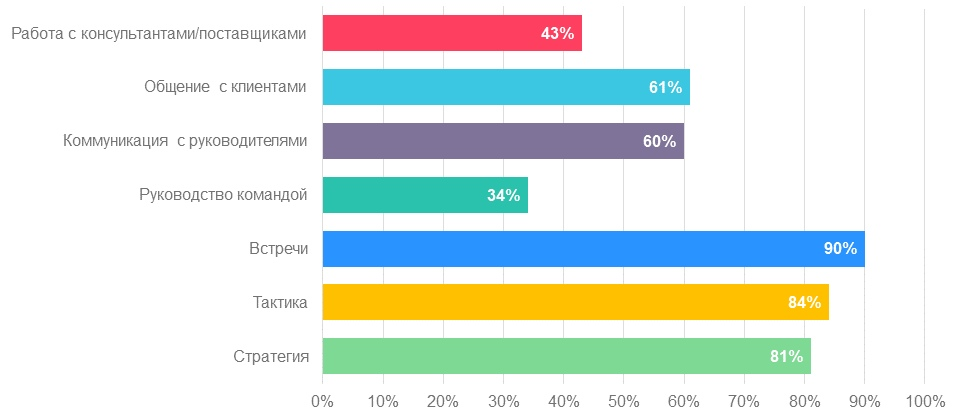
\includegraphics[width=1\linewidth]{day.png}}
\end{frame}
\lecturenotes


\begin{frame} \frametitle{Повседневные проблемы менеджера}
{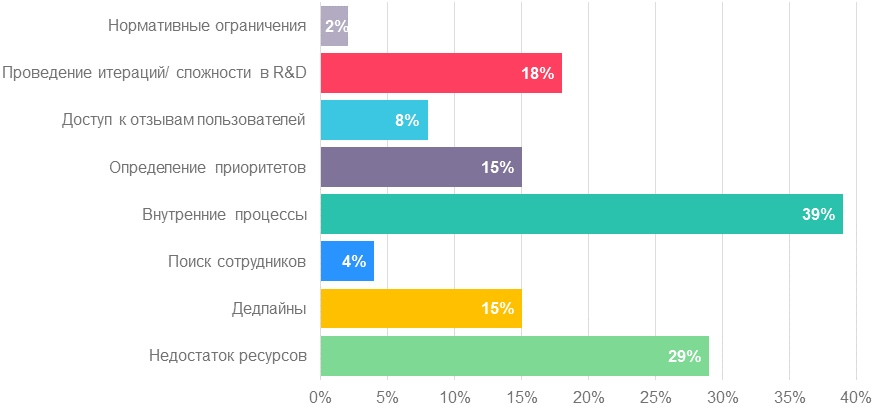
\includegraphics[width=1\linewidth]{problem.png}}
\end{frame}
\lecturenotes

\subsection{Планирование процесса}
\begin{frame} \frametitle{Планирование процесса}
Когда принято решение о разработке нового продукта, то на плечи менеджера ложится задача спланировать весь процесс работы над будущим проектом. Это касается таких вещей, как:
\begin{itemize}	
		\item Как будет выглядеть проект
		\item Сколько времени понадобится на проект
	 	\item Сколько именно средств придется выделить на проект, в каких местах можно сэкономить
	 	\item Какие специалисты будут задействованы в работе над проектом
		\item Как именно следует распределить задачи в команде
	 	\item Сколько будет стоить продукт, кто и как его будет продвигать на рынке

 \end{itemize}
\end{frame}
\lecturenotes

~\cite{How_to_be_a_good_IT-manager}

\subsection{Встреча с клиентом}
\begin{frame} \frametitle{Встреча с клиентом}
Для менеджера, проводящего первую встречу с возможным клиентом, основными целями являются:
\begin{itemize}	
		\item Оценка перспектив и готовности клиента к сотрудничеству
		\item Определение главных потребностей собеседника
	 	\item Выяснение, какие из товаров и услуг, предлагаемых вашей компанией, могут быть ему полезны и интересны
	 	\item Предложение пробников продуктов, показ образцов работ
		\item Получение обратной связи от клиента

 \end{itemize}
\end{frame}
\lecturenotes

~\cite{How_to_be_a_good_IT-manager}

\begin{frame} \frametitle{Ошибки при встрече с клиентом}
Менеджеры, выезжающие на личные встречи с клиентами – даже самые опытные и толковые – иногда ошибаются. Наиболее типичны следующие ошибки:
\begin{enumerate}

		\item Сразу презентовать свой товар (услугу), пропустив этапы вхождения в контакт и узнавания актуальных потребностей клиента. 
		\item Непонимание главной потребности клиента, смещение акцента внимания на менее важные нужды и проблемы, о которых он упомянул.
	 	\item Выражение неудовольствия действиями клиента (опозданием, переносом встречи, отказом и т. д.).
		\item Необдуманное предложение бонусов, скидок и других льготных условий для клиента.
	 
\end{enumerate}
\end{frame}
\lecturenotes

~\cite{How_to_be_a_good_IT-manager}


\begin{thebibliography}{99}
\bibitem{How_to_be_a_good_IT-manager} \href{http://www.pvsm.ru/upravlenie-proektami/36476}
\bibitem{Managers_in_IT} \href{https://habrahabr.ru/post/219741/}
\bibitem{Managers_thinking_style} \href{http://www.hr-asteri.ru/employer/poleznaya_informaciya/stil_myshleniya_i_povedeniya_professionalnogo_rukovoditelya/}
\bibitem{Programmer_vs_manager} \href{https://dou.ua/lenta/articles/programmer-vs-manager/}
\bibitem{Best_qualities_for_IT-manager} \href{http://hr-portal.ru/article/kakie-kachestva-nuzhny-menedzheru-it-proektov}
\bibitem{From_engineer_to_manager_keeping_your_technical_skills} \href{https://hackernoon.com/from-engineer-to-manager-keeping-your-technical-skills-40579cc8ea00}
\bibitem{From_programmer_to_manager} \href{https://m.dotdev.co/what-i-learned-transitioning-from-being-a-programmer-to-an-it-manager-8e58e7b406}
\end{thebibliography}

\end{document}

%%% Local Variables: 
%%% mode: TeX-pdf
%%% TeX-master: t
%%% End: 
